\documentclass[11pt, oneside]{article}   	% use "amsart" instead of "article" for AMSLaTeX format
\usepackage{geometry}                		% See geometry.pdf to learn the layout options. There are lots.
\geometry{letterpaper}                   		% ... or a4paper or a5paper or ... 
%\geometry{landscape}                		% Activate for for rotated page geometry
%\usepackage[parfill]{parskip}    		% Activate to begin paragraphs with an empty line rather than an indent
\usepackage{graphicx}				% Use pdf, png, jpg, or eps§ with pdflatex; use eps in DVI mode
								% TeX will automatically convert eps --> pdf in pdflatex		
\usepackage{amssymb}
\usepackage{amsmath}
\usepackage{parskip}
\usepackage{color}
\usepackage{hyperref}

\title{Pendulum and earth tunnel}
%\author{The Author}
%\section{}
%\subsection*{}
\date{}							% Activate to display a given date or no date

\graphicspath{{/Users/telliott_admin/Tex/png/}}
% \begin{center} 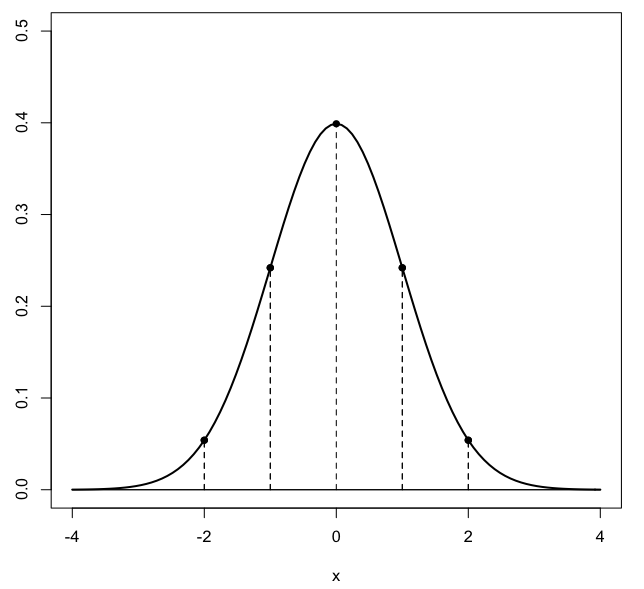
\includegraphics [scale=0.4] {gauss3.png} \end{center}
\begin{document}
\maketitle
\Large

A useful extension of the harmonic oscillator is to the problem of the pendulum.
\begin{center} 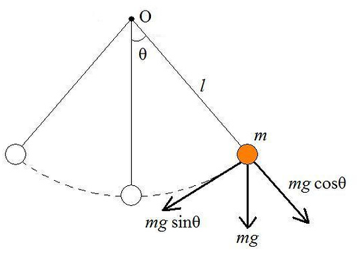
\includegraphics [scale=0.6] {pendulum1.png} \end{center}
The \emph{torque} on the mass is computed from the component of the gravitational force perpendicular to the rod, which is $-mg \sin \theta$

The vector components are drawn a bit too long in the figure, the total force should be the hypotenuse of a right triangle with sides $F \sin \theta$ and $F \cos \theta$.
\[ \tau = -mgL \sin \theta \]
We apply the small angle approximation $\sin x \approx x$ and obtain:
\[ \tau = -mgL \theta \]
Torque is related to angular momentum the way force is related to momentum
\[ \tau = I \ddot{\theta} \]
so
\[ I \ddot{\theta} + mgL \theta = 0 \]
This is exactly the equation we solved above.  In particular
\[ \omega = \sqrt{\frac{mgL}{I}} = \sqrt{\frac{mgL}{mL^2}} = \sqrt{\frac{g}{L}} \]
The period $T$ times the angular frequency is $2\pi$
\[ T \omega = 2 \pi \]
\[ T = 2 \pi \sqrt{\frac{L}{g}} \]
The period is independent of the mass.

\hypertarget{Earth_tunnel}{}

\subsection*{Tunneling through the earth}
Kline (Fig 10-18) has a fun problem.  

Imagine that  a tunnel has been bored straight through the earth between $U$ and $V$ in the figure and we consider the motion of a particle that is free to move through the tunnel --- maybe a railroad car on some kind of track.

\begin{center} 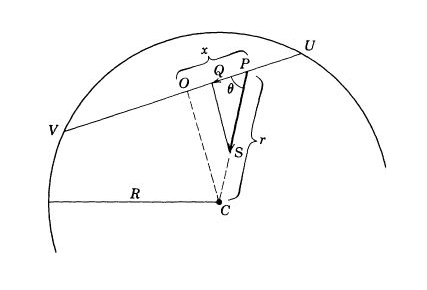
\includegraphics [scale=0.6] {earth_tunnel.png} \end{center}

The car will move under the force of gravity.  Kline does not derive it here, but the force inside the earth is variable depending on the position in the tunnel, partly due to the change in $r$, and partly due to the fact that the mass outside the current radius $r$ does not generate any net force.  Rather than the standard
\[ F = \frac{GmM}{r^2} \]
the formula is
\[ F = \frac{GmM}{R^3} r \]
Kline says, let $k = GM/R^3$ so
\[ F = kmr \]

We choose the coordinate system as shown, with the origin at the midpoint of the tunnel.  The effect of the force is to move the car along the tunnel, so we need to calculate the part of the force that points in that direction.  It is simply $F \cos \theta$, where $\cos \theta = x/r$.  Somewhat miraculously, with a nice cancelation, the force becomes
\[ F = kmx \]
We take $x$ positive to the right, while the force is in the negative $x$-direction so switch signs
\[ F = -kmx \]

Apply Newton's second law, obtaining a differential equation
\[ F = -kmx = m \ddot{x} \]
\[ -kx = \ddot{x} \]

We know the solution to this one.  The second derivative of the function is minus the function.  A general solution is
\[ x(t) = A \sin t + B \cos t \]
A factor of $\sqrt{k}$ is needed inside the trig functions:
\[ x(t) = A \sin (\sqrt{k} \cdot t) + B \cos (\sqrt{k} \cdot t) \]
Check by differentiating.  Now we use two initial conditions, one is that $v_0 = 0$.
\[ v_0 = \dot{x}(0) = A \sqrt{k} \cos (\sqrt{k} \cdot 0) - B \sqrt{k} \sin (\sqrt{k} \cdot 0) \]
At $t=0$, $\sin t = 0$, so we need the first term to be zero, with $A = 0$ and the equation reduces to
\[ x(t) =  B \cos (\sqrt{k} \cdot t) \]

The second is that $x(0) = x_0$ so $B = x_0$ and
\[ x(t) =  x_0 \cos (\sqrt{k} \cdot t ) \]
We have a periodic or oscillatory motion.  The period is
\[ T \sqrt{k}  = 2 \pi \]
\[ T = \frac{2 \pi}{\sqrt{k}} \]

We defined
\[ k = GM/R^3 \]
but recall that at the surface of the earth
\[ 32 m = \frac{mMG}{R^2} \]
\[ 32 = \frac{MG}{R^2} \]
so
\[ k = \frac{GM}{R^3} = \frac{32}{R} \]
and
\[ T = 2 \pi \sqrt{\frac{R}{32}} \]

With the radius measured in feet
\[ R = 3959 \cdot 5280  = 20903520 \]
\[ \frac{1}{\sqrt{k}} = 808.2 \]
$T = 5077$ seconds or about $85$ minutes.

It is very interesting that this result does not depend on the location or the length of the tunnel.

The fastest time occurs for a hypocycloidal path.

Kline: 

\begin{quote}The following data give some idea of what can be gained by using a hypocycloidal path. Suppose that a straight tunnel is dug between New York and San Francisco. Along the surface of the earth the two cities are about 2,575 miles apart, but the tunnel would be 2,530 miles long. At the midpoint the tunnel would be 206 miles below the surface; the maximum velocity acquired by the object, which would be at the midpoint, would be 1.57 mi/ sec; and a one-way journey, according to (reference), would take about 42 minutes. The hypocycloidal path would be 2940 miles long. At the midpoint the tunnel would be 820 miles below the surface; the velocity of the object at that point would be 3 mi/ sec; and the one-way journey would take 26 minutes.\end{quote}

\begin{center} 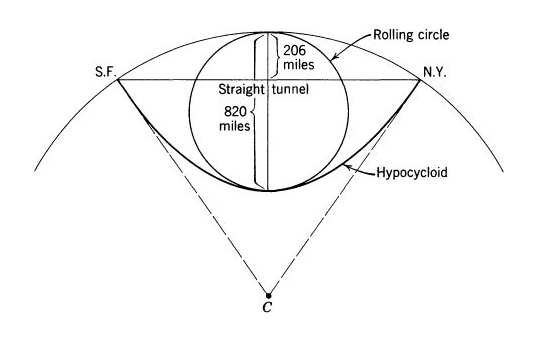
\includegraphics [scale=0.6] {earth_tunnel2.png} \end{center}

We can calculate the velocity for the straight line path.
\[ \dot{x}(t) =  -x_0  \sqrt{k} \sin (\sqrt{k} \cdot t) \]
which has a maximum when the sine term is equal to $1$ , at one-quarter and three-quarters of the period.
\[ |v_{\text{max}}| = x_0 \sqrt{k} = 1265 / 808 = 1.57 \text{ mi/sec} \]
which matches the text.

We can check the calculation another way, by using the conservation of energy.  We have that the potential energy lost is $mgh$ (it shouldn't matter that $g$ changes as we go inside the earth).  This is equal to the kinetic energy gained:

\[ \frac{1}{2} mv^2 = mgh \]
\[ v = \sqrt{2 \cdot 32 \cdot 206 \cdot 5280} = 8343 \text{ ft/sec} = 1.58 \text{ mi/sec} \]

Another angle is to ask how things would differ on the moon?  Given:

mass is $1/81$;  radius is $3/11$;  gravity is $1/6$.

$k$ goes like $M/R^3$ or $1/81 \times (11/3)^3 = 11^3/3^7$

$\sqrt{k}$ goes like 
\[ \frac{11 \sqrt{11}}{3^3 \sqrt{3}} = \frac{11 \sqrt{11}}{27 \sqrt{3}}  = 0.78 \]

Since $T$ is proportional to the inverse it's about $1.28$ times longer.  Not as much different as you might expect.


\end{document}  